\documentclass{article}
\usepackage{graphicx} % Required for inserting images
\usepackage[backend=biber]{biblatex}
\usepackage{listings}
\usepackage{subfigure}
\addbibresource{bibliography.bib}

\title{Machine Learning For Data Science I, \\[0.1cm] Homework 02}

\author{Maj Gaberšček, 27212075}
\date{March 2023}

\begin{document}

\maketitle

\section{Setup: a proxy for true risk}

First we generated the toy dataset of 100.000 rows. As we were coding this homework in \texttt{Python}, we had to write the \texttt{toy\_data} and the \texttt{log\_loss} functions from scratch. 


We generated 100.000 rows of data and stated that it is enough, to safely reduce the error to the first decimal digit. We can see this by estimating at the margin of error or standard error of the sample mean. \textbf{Margin of error} can be calculated as 
$$ME = \frac{z \cdot s}{\sqrt{n}},$$
where $s$ is the sample standard deviation, $n$ is the sample size and $z$ is the z-score (1.96 for 95\% confidence interval).
We want to have $ME < 0.0005$ (for accuracy to the 3rd decimal digit with 95\% confidence). We can also assume a large value for $s$, such as 0.5. If we insert the numbers, we can see, that $n=100000$ is enough to have $ME < 0.0005$.


\section{Holdout estimation}

\subsection{Model loss estimator variability due to test data variability}

In this part of the homework, we wanted to test our, how true risk of a model differs to estimated risk, calculated on test data. The output of my code is printed below and the plot of estimated risk differences is drawn in Figure \ref{fig:risk_differences_1}:

\begin{lstlisting}[basicstyle=\small\ttfamily]
True risk proxy:            0.4853
Mean difference:            0.0006
0.5-0.5 baseline true risk: 0.6399
Median standard error:      0.0592
Percentage of 95CI that contain the true risk proxy: 93.1
\end{lstlisting}

\begin{figure}
    \centering
    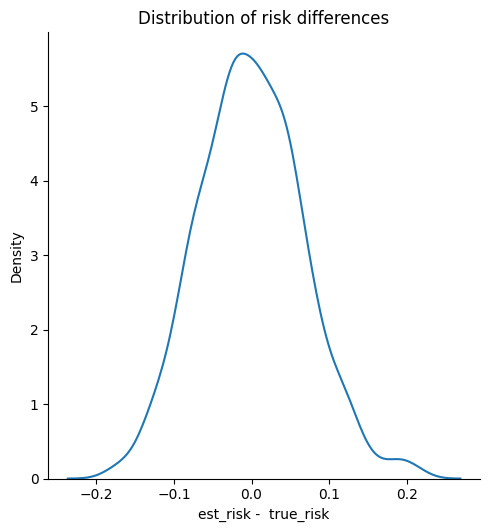
\includegraphics[width=0.5\textwidth]{homework-02/plots/risk_differences_1.png}
    \caption{Density estimate of the differences between estimates and the true risk proxy}
    \label{fig:risk_differences_1}
\end{figure}

From the results, we can conclude, that sometimes holdout estimation overestimates the risk and sometimes it underestimates it. The mean difference is very close to 0, from which we can see, that holdout estimation does indeed return expected risk same as the true one (if we performed estimation enough times, we could get as close as needed to true risk). So, in practice, we could estimate true risk proxy as accurately as needed by repeating this procedure more and more times.

If the training set would be bigger, mean difference would drop even more (because larger training set would learn the model more accurately). The median standard error of estimations would also decrease. Number of times, that the confidence interval contains the true risk proxy would also increase with larger testing set (as the training set would now represent the population even better). Similarly, with a smaller training set, the effect would be the other way around.

\subsection{Overestimation of the deployed model’s risk}

Here, we wanted to see, how the true risk calculated on model, which learned on 100 observations, differs to true risk of a model, which learned on a subset of this 100 observations of size 50. Results of true risk differences (model on smaller dataset minus model on bigger dataset), repeated 50 times, is copied below:

\begin{lstlisting}[basicstyle=\small\ttfamily]
Minimum:       -0.0349
1st Quantile:   0.0133
Median:         0.0322      
Mean:           0.0381        
3rd Quantile:   0.0666
Maximum:        0.1265  
\end{lstlisting}

We can see, that almost every time, we achieved better predictions (smaller risk), if testing on additional 50 data occurrences. If both datasets would be bigger (and difference in size would remain the same), the difference of risks would start to get smaller, as additional samples would not change the prediction that much (as population would already be well represented). Similarly, if both datasets were smaller, each individual training sample would contribute more towards final prediction, and differences in models' risks would be bigger.

\subsection{Loss estimator variability due to split variability}

Here, we generated a toy dataset of size 100, calculated a true risk proxy. Then we split the dataset into training and test and then trained another model on training data. We estimated original model's risk (model trained on data of size 100) by testing on test data. Code output was:

\begin{lstlisting}[basicstyle=\small\ttfamily]
True risk proxy:        0.4933
Mean difference:        0.0123
Median standard error:  0.0986
Percentage of 95CI that contain the true risk proxy: 97.8
\end{lstlisting}

We plotted difference between estimated risk and true risk in Figure \ref{fig:risk_differences_2}.

\begin{figure}
    \centering
    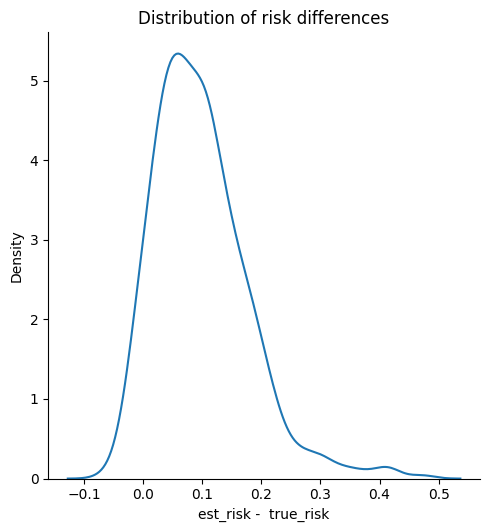
\includegraphics[width=0.5\textwidth]{homework-02/plots/risk_differences_2.png}
    \caption{Density estimate of the differences between estimates and the true risk proxy}
    \label{fig:risk_differences_2}
\end{figure}

We can conclude, that if the data would be bigger, estimated risk would also get closer to true risk. Mean difference and median standard error would decrease.

\section{Cross-validation}

In this section, we tested risk estimations with different kinds of cross-validations. Results of this experiment:

\begin{lstlisting}[basicstyle=\small\ttfamily]
----------------------------------------
Estimator: 2-fold cross validation
Mean difference:                                0.0438
Median standard error:                          0.0037
Confidence interval contains true risk proxy:   82.4%
----------------------------------------
Estimator: leave-one-out cross validation
Mean difference:                                0.0017
Median standard error:                          0.0027
Confidence interval contains true risk proxy:   91.2%
----------------------------------------
Estimator: 10-fold cross validation
Mean difference:                                0.0068
Median standard error:                          0.0028
Confidence interval contains true risk proxy:   90.0%
----------------------------------------
Estimator: 4-fold cross validation
Mean difference:                                0.0174
Median standard error:                          0.0030
Confidence interval contains true risk proxy:   87.6%
----------------------------------------
Estimator: 10-fold cross validation repeated 20 times
Mean difference:                                0.0061
Median standard error:                          0.0027
Confidence interval contains true risk proxy:   32.0%
\end{lstlisting}

If we compare different estimators, we can conclude, that 2-fold cross validation generated biggest mean difference in comparison to other estimators, as well as the biggest standard error. Best model in terms of mean difference and also median standard error is leave-one-out, which was well expected. However, for practical purposes, it is important to point out, that leave-one-out model is by far the most time consuming one. 

If we compare 10-fold cross validation and 10-fold cross validation repeated 20 times, we can see almost no difference in term of median standard error or mean difference.

Plots of risk differences can be seen in Figures \ref{fig:cross-fold}

\subsection{A different scenario}

I did not code this part of the exercise. 

\begin{figure}
    \centering
    \subfigure[2-fold]{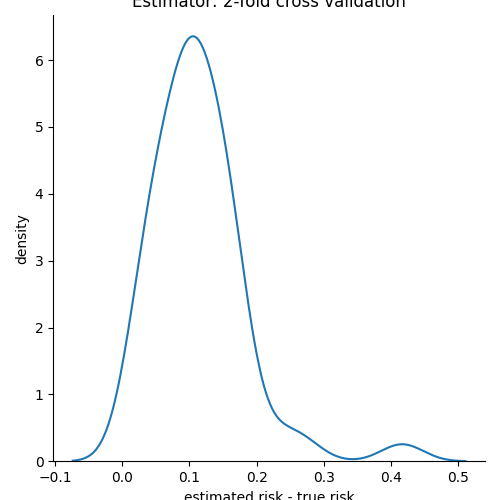
\includegraphics[width=0.4\textwidth]{homework-02/plots/estimator_2-fold.png}}
    \subfigure[4-fold]{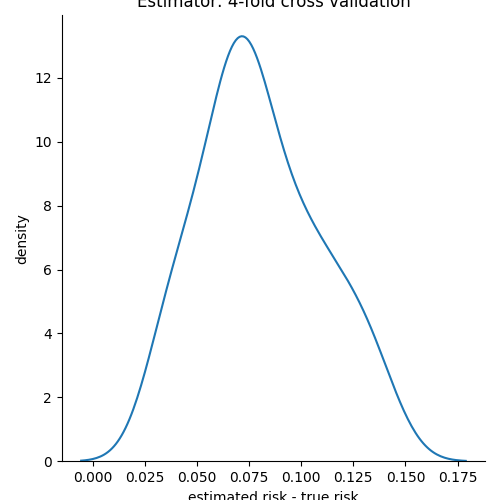
\includegraphics[width=0.4\textwidth]{homework-02/plots/estimator_4-fold.png}}
    \subfigure[10-fold]{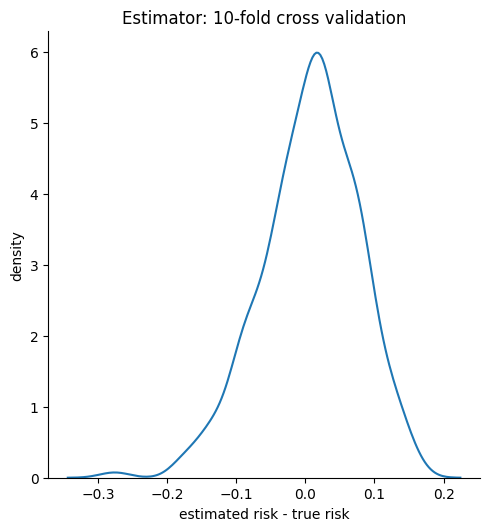
\includegraphics[width=0.4\textwidth]{homework-02/plots/estimator_10-fold.png}}
    \subfigure[20 times 10-fold]{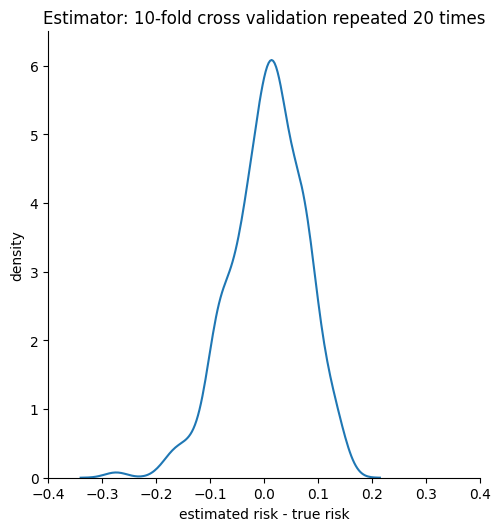
\includegraphics[width=0.4\textwidth]{homework-02/plots/estimator_20-10-fold.png}}
    \subfigure[leave-one-out]{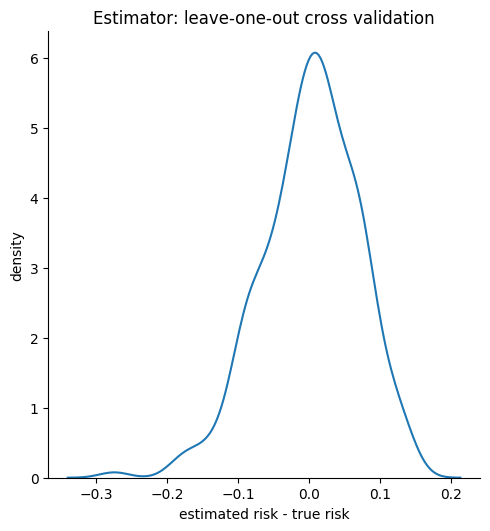
\includegraphics[width=0.4\textwidth]{homework-02/plots/estimator_leave-one-out.png}}
    \caption{Density estimate of the differences between estimates and the true risk proxy}
    \label{fig:cross-fold}
\end{figure}


\printbibliography

\end{document}